\section{Erster Lösungsansatz
\label{perturbation:section:ersterloesungsansatz}}
\rhead{Erster Lösungsansatz}

Die Formeln \ref{eq:x_simple} und \ref{eq:y_simple} sind ohne viel Rechenleistung berechenbar und somit auch als Flugobjekt durchführbar. Die Störungstheorie befasst sich damit, die Starparameter $x_0$, $y_0$, $v_{0_x}$ und $v_{0_y}$ so abzuändern, dass dennoch gute Approximationen für $x(t)$ und $y(t)$ gefunden werden können. Hierbei ist es die Aufgabe der Bodenstation, die notwendigen Startparameter dem Flugobjekt mitzuteilen, sodass dieses die Berechnung auf Basis der trivialen Formeln \ref{eq:x_simple} und \ref{eq:y_simple} vornehmen kann.

Als ersten Lösungsansatz haben wir $v_{0_x}$ und $v_{0_y}$ durch lineare Funktionen abhängig von der Zeit ersetzt, aber $x_0$ und $y_0$ vorerst unberührt gelassen. Hintergrund dieser Überlegung ist, dass der Luftwiderstand ja nur die Geschwindigkeit beeinflusst.
\[
v_{0_x} \rightarrow v_{0_x}(t) = v_{0_x} + \nu_x \cdot t
\]
\[
v_{0_y} \rightarrow v_{0_y}(t) = v_{0_y} + \nu_y \cdot t
\]

Wir passen die Startgeschwindigkeit im Verlaufe der Zeit $t$ also anhand eines unbekannten Faktors $\nu$ an. Eingesetzt in die Formeln \ref{eq:x_simple} und \ref{eq:y_simple} erhalten wir:
\begin{equation}\label{eq:x_linear}
    x(t) = x_0 + t \cdot (v_{0_x} + \nu_x \cdot t)
\end{equation}
\begin{equation}\label{eq:y_linear}
    y(t) = y_0 + t \cdot (v_{0_y} + \nu_y \cdot t) - \frac{1}{2}gt^2
\end{equation}

$x_0$, $y_0$, $v_{0_x}$ und $v_{0_y}$ sind die bekannten Anfangsbedingungen des Problems. Ebenfalls können $x(t)$ und $y(t)$ mit dem Runge Kutta Verfahren bestimmt werden, wie in Kapitel \ref{chapter:numerische_lsg} beschrieben. Um neue Werte mit der Störung zu bestimmen, müssen die Unbekannten $\nu_x$ und $\nu_y$ berechnet werden. Diese können bestimmt werden, in den man die Gleichungen \ref{eq:x_linear} und \ref{eq:y_linear} nach $\nu_x$ bzw. $\nu_y$ auflöst:
\[
\nu_x = \frac{x(t) - x_0 - tv_{0_x}}{t^2}
\]
\[
\nu_y = \frac{y(t) - y_0 - tv_{0_y} + \frac{1}{2}gt^2}{t^2}
\]

Beispielsweise kann dieses Gleichungssystem für $t = 5s$ gelöst werden. Dadurch erhält man $\nu_x$ und $\nu_y$. Da hierzu allerdings $x(t=5)$ und $y(t=5)$ mittels Runge-Kutta berechnet werden müssen, ist dazu nur die Bodenstation in der Lage. Die Werte $\nu_x$ und $\nu_y$ können nun aber dem Flugobjekt übertragen werden, welches mit den Formeln \ref{eq:x_linear} und \ref{eq:y_linear} seine Position in naher Zukunft nun autonom approximieren kann, beispielsweise für das Intervall $t \in [5,6)$. Anschliessend könnte die Bodenstation die Werte $\nu_x$ und $\nu_y$ für $t=6s$ neu berechnen, um den Fehler nicht beliebig anwachsen zu lassen.

Geplottet ergibt dies das Resultat in Abbildung \ref{naive_linear_term}. Rot ist das dabei das nummerische Resultat der Differentialgleichungen \ref{eq:x_diff} und \ref{eq:y_diff}, blau ohne eingesetzte lineare Funktion und türkis die korrigierte Variante. Für die korrigierte Variante wurde eine Intervalllänge von $t=1s$ gewählt. Das heisst, sie bestimmt die Unbekannten $\nu_x$ und $\nu_y$ zu jeder vollen Sekunde $t \in \{1, 2, 3, \cdots, 25\}$ und nutzt jene Daten, um die Position jeweils eine Sekunde später vorherzusagen. Wie zu erkennen ist kann ein Grossteil des Fehlers bereits vermieden werden.
\begin{figure}
    \centering
    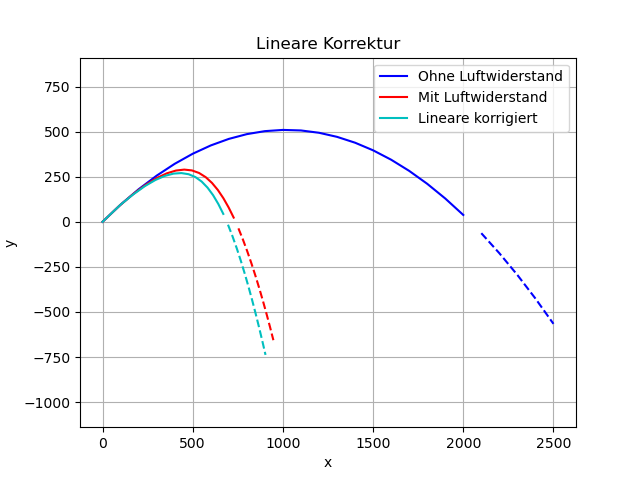
\includegraphics[scale=0.7]{papers/perturbation/bilder/img1.png}
    \caption{Linearer Korrekturterm}
	\label{naive_linear_term}
\end{figure}


Anstelle des linearen Ansatzes könnte man auch einen quadratischen Ansatz nutzen. Dies ergibt anstelle von \ref{eq:x_linear} und \ref{eq:y_linear}:
\begin{equation}
    x(t) = x_0 + t \cdot (v_{0_x} + \nu_{x_1}t + \nu_{x_2}t^2) = x_0 + v_{0_x}t + \nu_{x_1}t^2 + \nu_{x_2}t^3
\end{equation}
\begin{equation}
    y(t) = y_0 + t \cdot (v_{0_y} + \nu_{y_1}t + \nu_{y_2}t^2) - \frac{1}{2}gt^2 = y_0 + v_{0_y}t + \nu_{y_1}t^2 + \nu_{y_2}t^3 - \frac{1}{2}gt^2
\end{equation}

Damit haben wir noch bessere Resultate erhalten. Diese sind in Abbildung \ref{naive_quadratic_term} ersichtlich. Von Auge ist bereits kein Unterschied der beiden Flugbahnen mehr erkennbar.
\begin{figure}
    \centering
    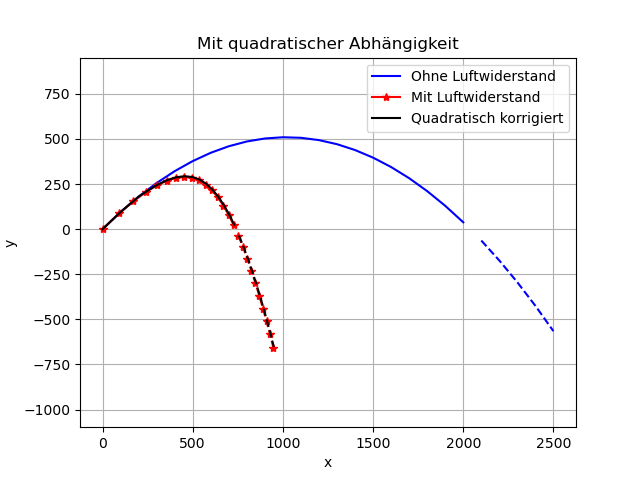
\includegraphics[scale = 0.7]{papers/perturbation/bilder/img2.png}
    \caption{Quadratischer Korrekturterm}
	\label{naive_quadratic_term}
\end{figure}